\documentclass[12pt]{article}
\usepackage{graphicx}
\usepackage{amsmath}
\usepackage{latexsym}
\usepackage{amstext}
\usepackage{array}
\usepackage{multirow}
\usepackage{stackrel}
\usepackage{caption}
\usepackage{subcaption}

%%%%%%%%%%%%%%%%%%%%%%%%%%%%%%%%%%%%%%%%%%%%%%%%%%%%%%%%%%%%%%%%%%%%%%%%%%%=
\newtheorem{proposition}{Proposition}
\newtheorem{lemma}{Lemma}
\newtheorem{theorem}{Theorem}
\newtheorem{corollary}{Corollary}
\newcommand{\Proof}{\underline{\bf Proof:}}
\newcommand{\Endproof}{~$\Box$~}
\newcommand{\mb}[1]{ \mbox{\boldmath$#1$} }
\newcommand{\ds}{\displaystyle}
\newcommand{\beq}{\begin{eqnarray}}
\newcommand{\eeq}{\end{eqnarray}}
\newcommand{\beqq}{\begin{eqnarray*}}
\newcommand{\eeqq}{\end{eqnarray*}}
\newcommand{\p}{\partial}
\newcommand{\g}{\gamma}
\newcommand{\eps}{\varepsilon}
\newcommand{\x}{\mbox{\boldmath$x$}}
\newcommand{\n}{\mbox{\boldmath$n$}}
\newcommand{\J}{\mbox{\boldmath$J$}}
%\newcommand{\v}{\mbox{\boldmath$v$}}
\newcommand{\y}{\mbox{\boldmath$y$}}
\newcommand{\z}{\mbox{\boldmath$z$}}
\font\bb=msbm10 at 12pt
\def\rR{\hbox{\bb R}}
\def\rN{\hbox{\bb N}}
\def\rQ{\hbox{\bb Q}}
\def\rZ{\hbox{\bb Z}}
\pagestyle{plain}
%%%%%%%%%%%%%%%%%%%%%%%%%%%%%%%%%%%%%%%%%%%%%%%%%%%%%%%%%%%%%%%%%%%%%%%%%%%%
\begin{document}

\title{Chromatin reconstruction and dynamics using random Loops accounting for Chromosome Capture data}
\author{O. Shukron,  L. Giogetti, E. Heard and D. Holcman$^{1}$ \footnote{ $^1$Ecole Normale Sup\'erieure, IBENS, 46 rue d'Ulm 75005 Paris, France.}}
\date{\today}
\maketitle
%%%%%%%%%%%%%%%%%%%%%%%%%%%%%%%%%%%%%%%%%%%%%%%%%%%%%%%%%%%%%%%%%%%%%%5
\begin{abstract}\label{abstract}
\end{abstract}
{\bf \noindent Keywords: Modeling, Inverse problem, First passage times,}\\

\section{Introduction}\label{section_introduction}
%> The relationship between chromosomal spatio-temporal organization and chromosomal activity is incompletely understood
[Unfinished]\\
The spatio-temporal organization of the chromatin plays an essential role in the regulation of sub-cellular activity such as gene expression\cite{cremer2001chromosome}.

%> Dynamic looping events between enhancer and promoters (like) are frequent in the nucleus and are related to the chromosomal dynamic organization

%> Chromosome Capture method creates loci contact maps, which are used to record chromosomal static looping events

%> Static looping events, coupled with dnamic polymer models, can shed light on the chromosoamal spatio-temporal organization

%> previous work on the subject
3d structure of the Igh locus was suggested by \cite{jhunjhunwala20083d} after tagging several position along the loci.

%> our work

\section{Experimental data and Methods}\label{section_experimentalDataAndMethods}

\subsection{The experimental data}\label{subsection_theExperimentalData}
%> The experimental data from 5c experiments includes a subset of 2 TADs out of the Nora et al data,we use the average data
We used the experimental 5C data generated by Nora et al.\cite{Nora2012} for the chromosome contact frequencies of the X chromosome in a 4.5 Gb region encompassing the X inactivation center. In our work we focused on a subset of the data, including a 94,082 bp region, termed TAD D and E (see \cite{Nora2012}).
Two replicates of the experiments were conducted. In our analysis we use the average of these two experimental replicates.

%> coarse graining of the data, following Giorgetti et al. allows for uniform bead spacing representation
The encounter histograms generated by the 5C experiments describes the contact between genomic loci of variable sizes over millions of nuclei. To map these contact into uniform sized segments, we followed data coarse-graining as described in \cite{Giorgetti2014}, to map segment encounter frequencies to that of evenly spaced, equal size beads. A bead size of 3000 bp was chosen according to the mean size of restriction segments resulted by HindIII enzyme digestion, used in the process of the 5C experiments \cite{Nora2012} \cite{Giorgetti2014} (Supplementary Materials). This choice of bead size resulted in coarse-grained polymer of 307 beads.

%> we use the coarse-grained representation to calculate bead encounter probability
The coarse-grained bead encounter frequencies includes 14,509 data points and was used to calculate the bead encounter probability as a function of the distance in beads units. For each bead, equidistant encounter frequencies were averaged, and the resulting encounter frequency signal was divided by the total number of encounters, to get the encounter probability as a function of bead distance.

%> fitting the experimental encounter probability with an analytical function
For each bead $n=1..307$ we fit the experimental encounter probability signal with a function of the form 
\begin{equation}\label{equation_encounterProbabilityModel}
p_n(d)=\alpha_n d^{-\beta_n}
\end{equation}
with $p_n$ the encounter probability of bead $n$, $\alpha_n = \frac{1}{\sum_{j=1}^k j^{-\beta_n}}$, $d$ is the distance in bead units, and $\beta_n$ is a parameter to be determined by the fitting procedure.


\subsection{The polymer model}\label{subsection_thePolymerModel}
%> Rouse polymer is used to represent the chromosome
To represent the chromosome polymer and to explore the different architectures that can explain the appearance of the TADs, we chose to use the Rouse chain. The Rouse chain describes the dynamics of a linear polymer as a collection of massless beads connected by harmonic springs and driven by the thermal forces of diffusion. The corresponding system of stochastic differential equations describing the time progression of a chain of $N$ beads is given, in the 3-dimensional case, by
\begin{equation}
\frac{dR}{dt}=-\frac{3D}{b^2}KR +\sqrt{2D}\frac{dW}{dt}
\end{equation}
where, $R(t)=[R_1(t),R_2(t),..,R_N(t)]^T$ describes the 3D coordinates of $N$ beads at time $t$, $D$ is the diffusion constant, $b$ is the standard-deviation of the distance between adjacent beads of the chain, $W$ is an independent $N\times3$ Brownian motion with mean 0 and variance 1 in each component, and $K$ is the Kirchhoff bead connectivity matrix, which reflects different chain connectivities.

%> polymer with random loops were tested to give rise to the TADs
We have constructed our polymer model to have $L$ loops of random sizes. To form each loops, we have randomly chosen 2 non-neighboring beads and altered the connectivity in the Kirchhoff matrix, with the condition that no bead can be connected to form more than one loop.

\subsection{Simulations}\label{subsection_simulations}
%> for each number of loops of variable size,
Throughout simulations, for each fixed number of loops, the chosen beads to connect varied randomly. Such a choice was made to refer to the heterogeneity if the spatial organization inside TAD between cells, even in the same cell phase \cite{Nora2012}.

%> simulation is done until relaxation time
Simulations were always carried out until the chain's relaxation time, in which point any two beads were determined to have encountered if their distance satisfied $|R_j-R_k|<\epsilon<b,\quad  (j\ne k)$.
The chain's relaxation time is given by the slowest mode of the linear chain
\begin{equation*}
\tau =\frac{b^2}{12D\sin(\frac{\pi}{2N})}
\end{equation*}
for which the number of simulation steps performed is $\frac{\tau}{\Delta t} $. The time step, $\Delta t$ was set so to prevent simulation 'blow-ups' by demanding that the quotient of the norms of beads position at two subsequent time steps would be smaller that unity, which resulted in $\Delta t < \frac{b^2}{12D}$.

%> fitting the simulation data and comparing to the theory to experimental data
For each tested polymer connectivity we constructed the bead encounter frequencies histogram and derived the bead encounter probability from it. The bead encounter probability was then fitted similarly to the fitting in eq. \ref{equation_encounterProbabilityModel}.

%> interpertation of the mean beta value
For a linear Rouse chain, the expected value of $\beta$ is $1.5$ \cite{doi1986theory}. We interpret $\beta<1.5$ as long range interaction resulting from non nearest-neighbor bead interactions.
Because the addition of non-neighboring connections to the linear chain can only increase the long range encounter probability, we have focused on interpreting the fitted values in the range $\beta<1.5$.

%> transfroming to normal coordinates

%> previous results of the MFPT (Amitai 2012)

%> the prcess of obtaining the MFET from the normal coordiantes linear chain case
%1. transfrom from spatial coordinates to normal coordinates
%2. solve the fokker planck equation (find suitable boundary conditions)
%3. express the solution as an infinite series
%4. integrate to get the CDF and calculate the survival function
%5. integrate the survival function to get the MFET




\section{Results}\label{section_results}
%> for the case of TAD D+E, beta value is below 1.5 which indicates long range interactions
\subsection{Analysis of the experimental data}\label{subsection_analysisOfTheExperimentalData}

%> calculation of the beta values by bead and the mean values will allow us to infer on structure.
To evaluate the mean encounter probability in the experimental data, we have calculated the $\beta$ value for the 3 cases of TAD D, TAD E and TAD D+E for each of the beads in those genomic region. This provides us with a basis for comparison of the results of simulations with the experimental data and to the inference on the spatial organization of the chromosome.

%> beta values by beads for the case of TAD D+E shows a pattern correlated with the TADs location and is inline with the expected beta
The calculation of $\beta$ for each bead in the case of TAD D+E resulted in a pattern which was aligned with the significant long range interactions (Figure \ref{figure_TADDAndENoraEtAl2012} b), represented by the peaks the encounter probability graph (Figure \ref{figure_encounterProbabilityTADDAndE+fittedBeta}). Indeed, the mean $\beta$ value was 0.729, which is well below the expected value for the linear Rouse chain (Figure \ref{figure_TADDAndENoraEtAl2012} c).

%>  Long range interactions are contributed by TAD E and inter-TAD interactions.
We then turned to examine whether long range interactions stem from inter or intra-TAD polymer looping.TAD D has almost no significant long range interactions (supplementary material), although the mean fitted $\beta$ value was 0.71, which indicates either packed organization of TAD D or heterogeneity of the location of loops within the cell population examined in the 5C experiments.
Intra-TAD long range interaction within TAD E contribute about half of the significant long range encounter peaks in the encounter probability graph (supplementary material), whereas the other half stem from inter-TAD long range interactions.

%> we turn to search for the polymer architecture which gives rise to the experimental observations
Given the calculation of the $\beta$ values from the experimental data we now turn to explore which polymer architecture give rise to the observations.

\subsection{Random fixed loops simulations}\label{subsection_randomFixedLoopsSimulations}
%> Placing loops corresponding to the peaks of the encounter data does not rescreate the observed values extracted from the experimental data
To examine if fixed loops in the polymer can recreate the TADs, we have placed connection between beads corresponding to the peaks of the encounter probability and simulated our model until relaxation time.
In a 307 beads polymer, these fixed loops were insufficient to recreate a TAD-like structure.
Only localized nearest neighbors interactions emerged by this model(Figure \ref{figure_encounterProbabilityPeaksOfTheEncounterData}) which cannot account for the observed long range interaction map.

%> strong peaks at the boundaries of TADs might indicate the presence of stable loops
Although these fixed loops are insufficient by themselves to create the encounter maps expected, we noticed peaks on the boundaries of TADs. We have postulated that these peaks, which connects the two boundaries of a TAD, are of significance to the spatial organization and the functionality of regulatory elements within the TAD.  We therefore set to examine the encounter probability of a polymer having a large fixed loop between two predefined ends.

% random positions of loops reflects the heterogeneity in internal organization within TAD of different cells
Furthermore, to reflect the heterogeneity in the spatial organization of the chromatin of cells in the HiC experiment \cite{dekker2013exploring} \cite{Nora2012}, we have added loops between randomly chosen beads on the linear chain between the two boundaries we have determined for the big loop (Figure \ref{figure_encounterProfileOneTADWithTails} a).

%> experiments with one TAD
Increasing the number of internal random loops from 1 to 10, we see an encounter pattern which resembles that of a TAD (Figure \ref{figure_encounterProfileOneTADWithTails}).

%> experiment with two TADs
Next, we added a second, adjacent region, to form a loop, and sequentially added 1 to 10 internal random fixed loops in each. (Figure \ref{figure_encounterProfileTwoTADs} ) %\textcolor{green}{[simulation have to be redone]}


%> show that the data contains peaks that might correspond to hard coded big loops
%> analyze the region containing the big loop in term of eigenvalues
%> analyze the normal coordinate system to find the encounter probability
%> show that the encounter probability beta value drops quadratically with the number of internal dynamic random loops
%> show the connection between the average beta and the average number of loops
%> argue that in the resultion of data that we have, we can only say something concrete about the large loop.
%> try to find the connection between gene expression and the number of loops the model predicted
%> try to estimate gene expression rate according to the encounter probability


\section{Discussion}\label{section_discussion}

\section{Figure}\label{section_figures}

\begin{figure}[H]
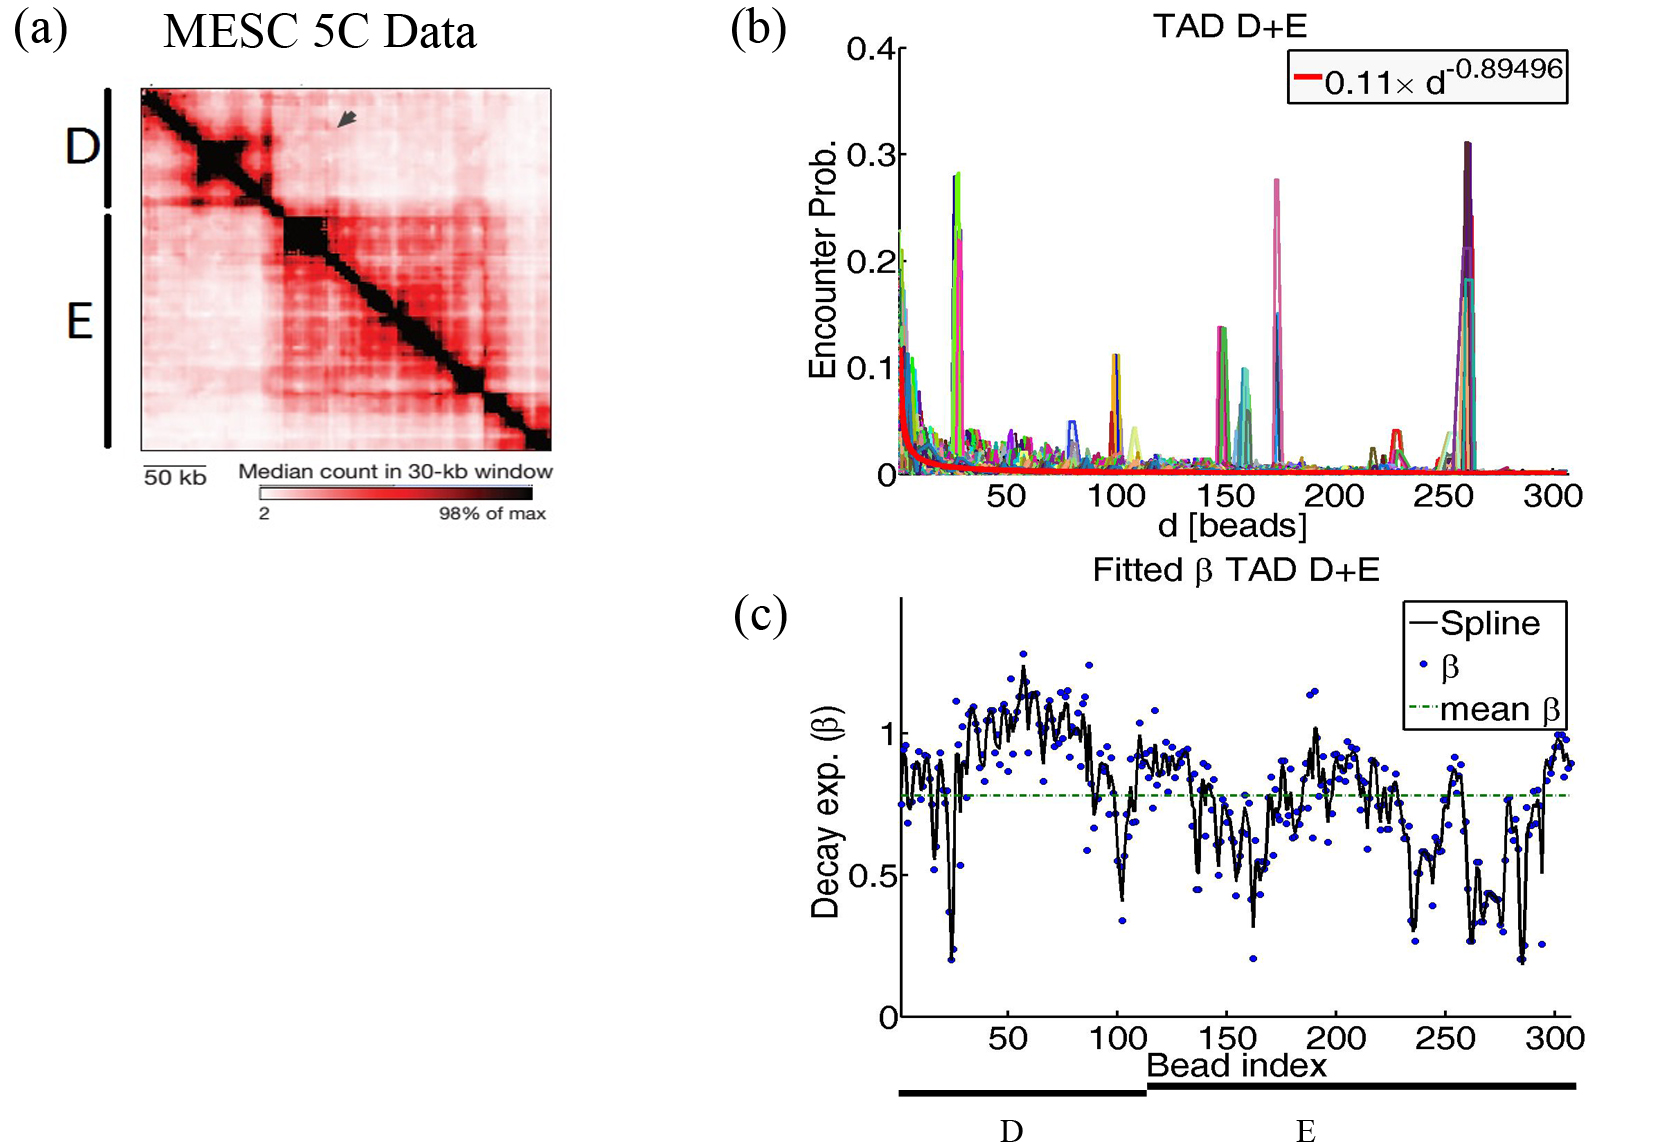
\includegraphics[scale=0.7]{Figure01_AnalysisOfTheExperimentalData}
\caption{\textbf{Analysis of the experimental data} (A) Average contact histogram of the 2 replicates of the 5C experiments in 2 discrete genomic regions of high self interactions termed TAD D and E (Nora et al \cite{Nora2012}) (B) The encounter probability graphs for each of the 307 beads show long range interactions between beads in TAD E and between TAD D and E, a fit of the form $\alpha d ^{-\beta}$ to the mean encounter of each distance (red curve), was found to have $\beta=0.729$, well below the expected $\beta=1.5$ for a linear Rouse polymer, implying compact configuration of the polymer and looping (C) The calculated $\beta$ value for each of the 307 beads (circles) was fitted with a smoothing spline (black curve) to show a fluctuating pattern around the mean ($\beta=0.729$, green dashed line) with sharp decrease in values for beads having long range interactions, e.g beads 25, 102, 165, 285.}
\label{figure_TADDAndENoraEtAl2012}
\end{figure}

\begin{figure}[H]
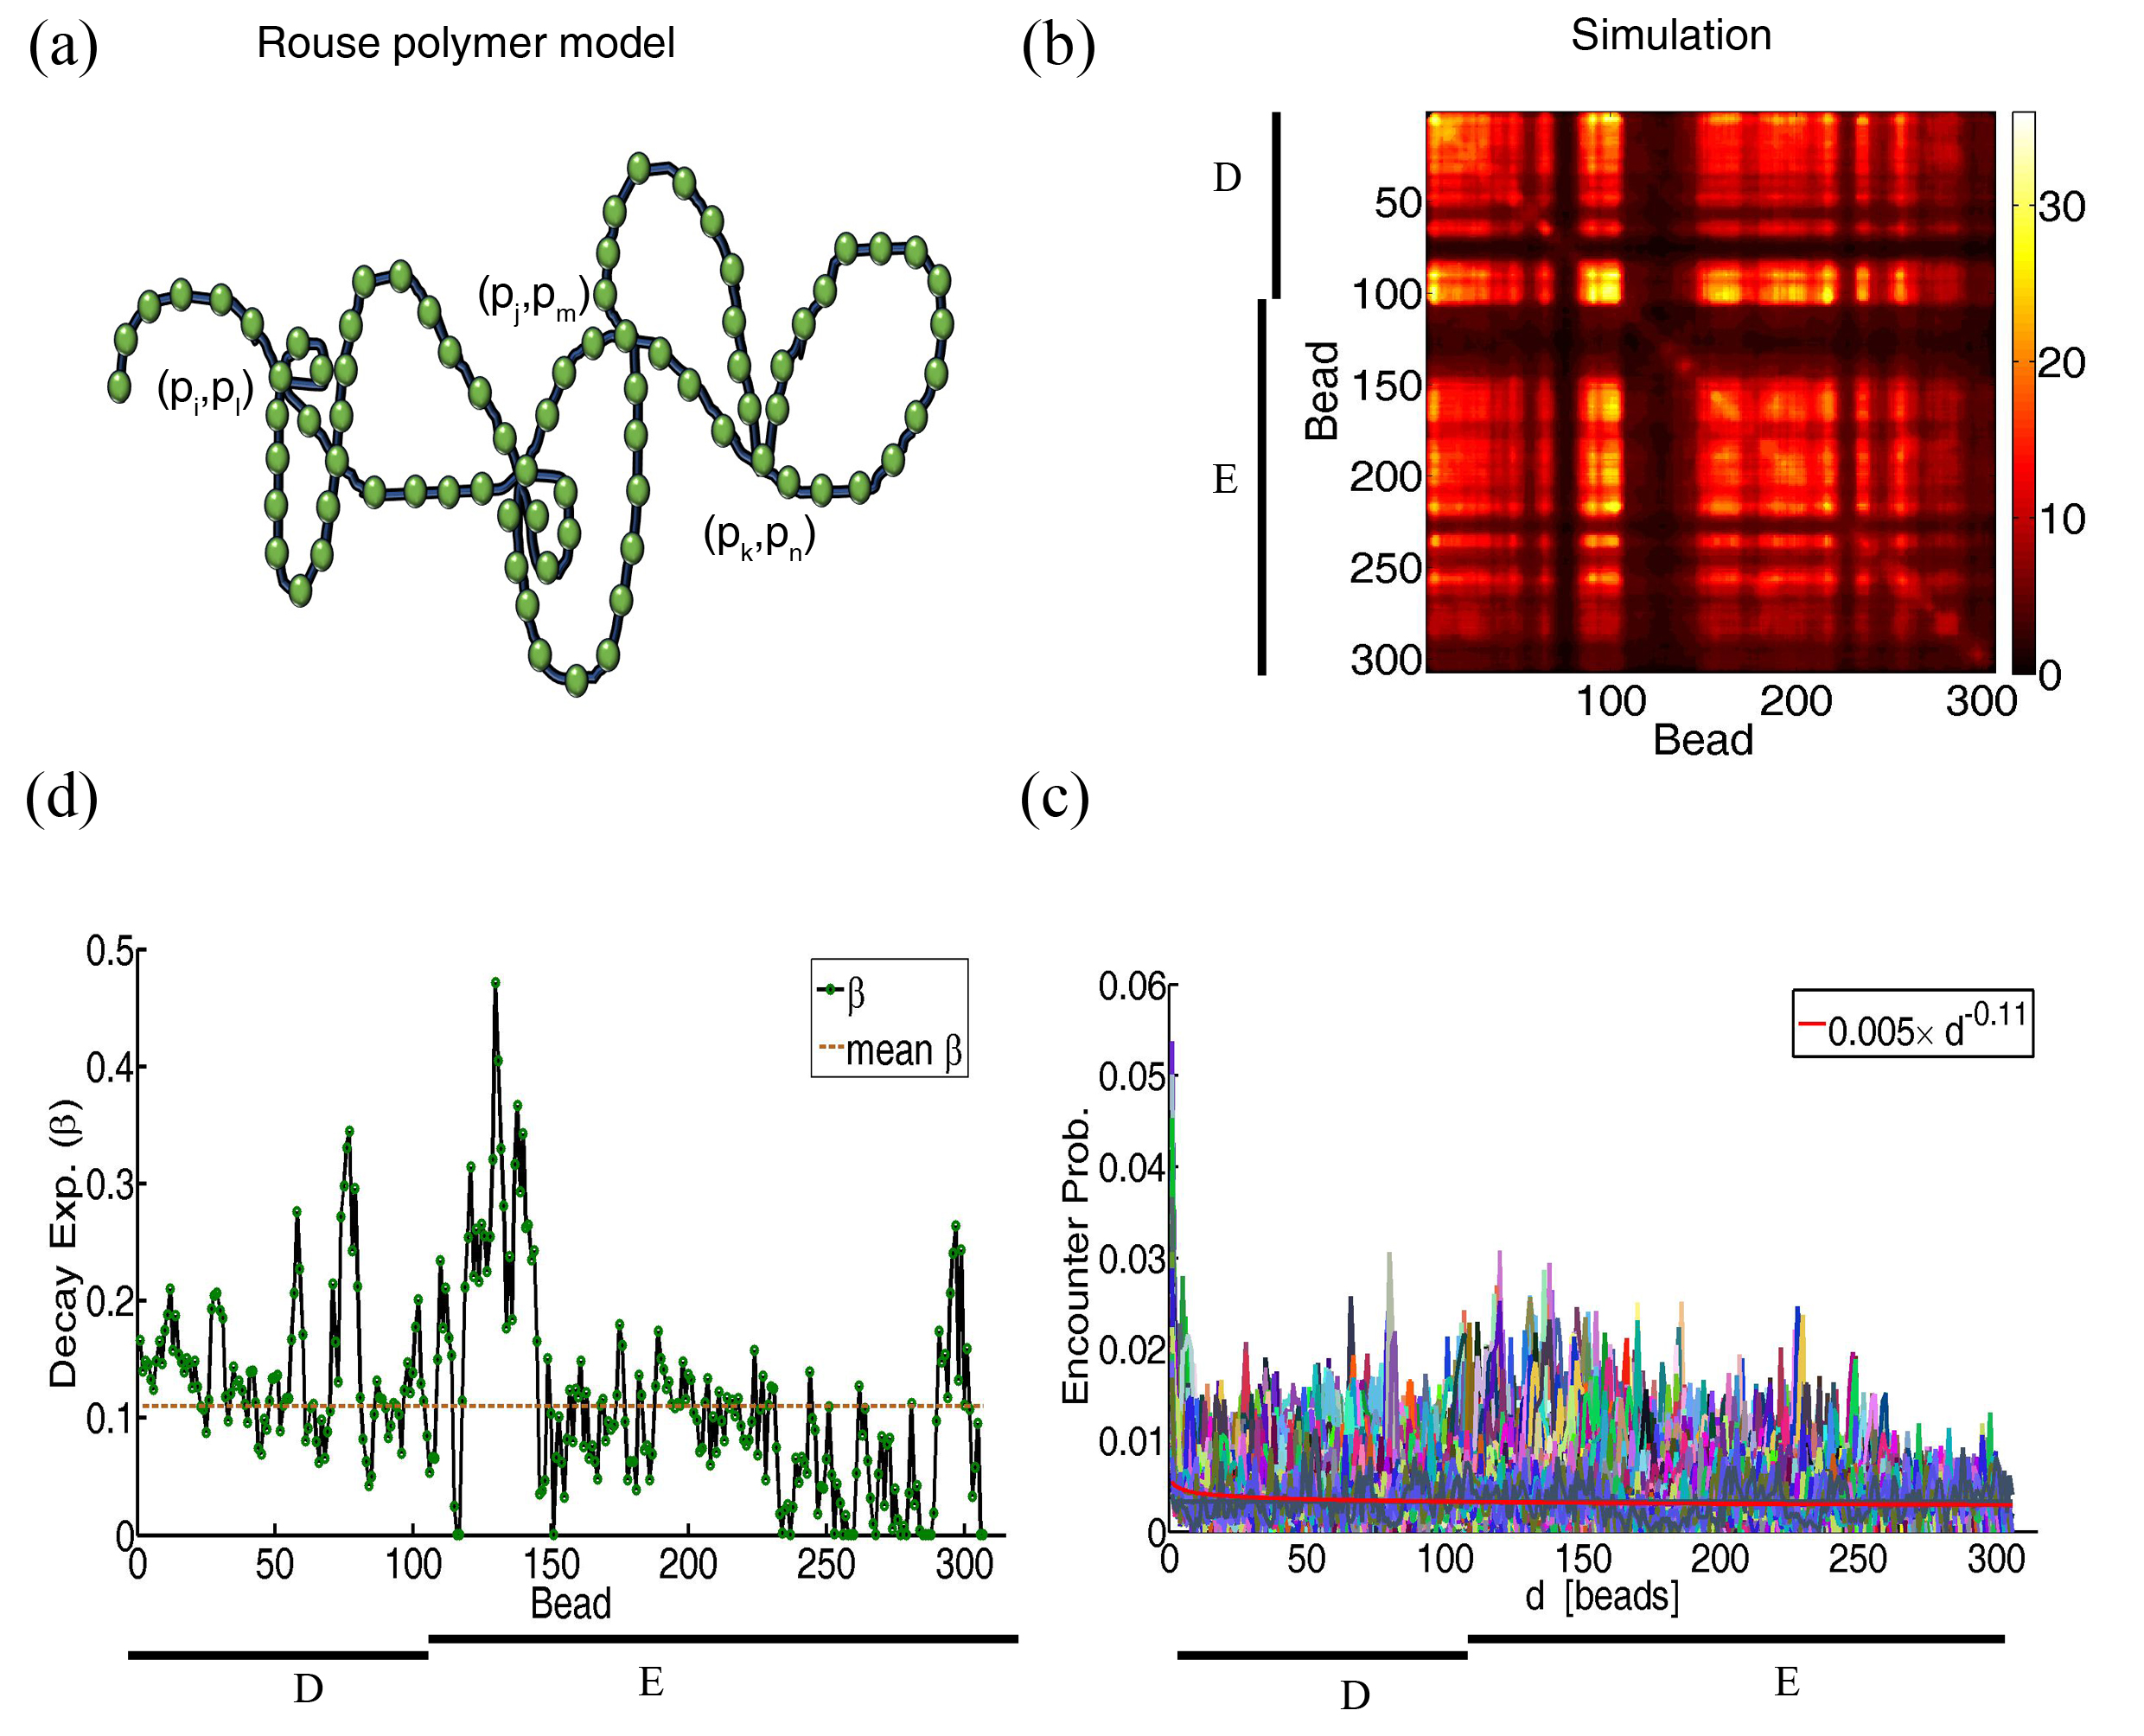
\includegraphics[scale=0.7]{Figure02_LoopsCorrespondingToPeaks307Beads}
\caption{\textbf{Simulation of a chain with connectors between beads displaying peaks of the encounter data}. (A) An illustration of a polymer connected between beads displaying peaks in the encounter data (B) The encounter histogram of the polymer with connectors does not show similarity to encounter histogram of the experimental data (Figure \ref{figure_TADDAndENoraEtAl2012}) (C) the encounter probabilities of all beads in of the simulated chain shows flat profile which resulted from the compact configuration of the polymer with connectors. (D) the fitted$\beta$ values for each one of the profiles in box (C) display low value corresponding to long range interaction of beads along the chain in the simulated polymer.)}
\label{figure_encounterProbabilityPeaksOfTheEncounterData}
\end{figure}

\begin{figure}[H]
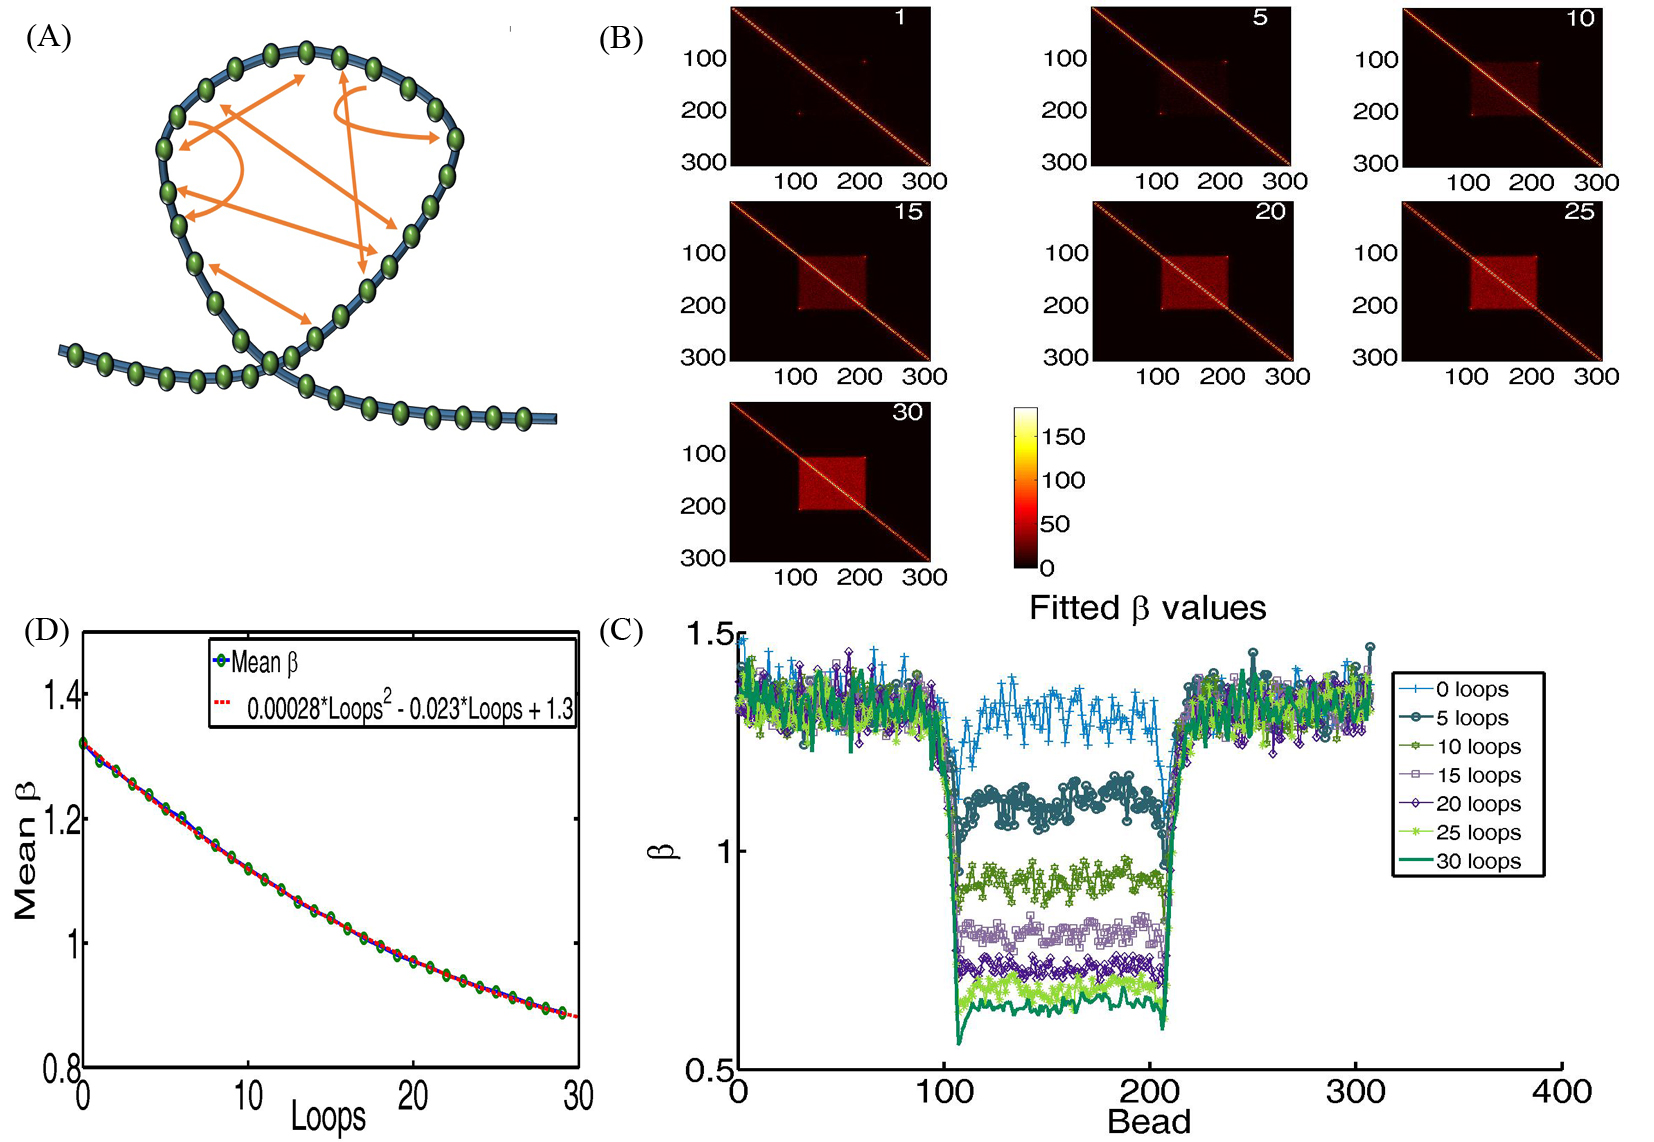
\includegraphics[scale=0.7]{Figure03_OneTADWithTails0To30RandomLoops}
\caption{\textbf{Encounter profile for a polymer model with one fixed loop and 1-30 random internal loops.} (A) A sketch of the polymer model used in simulation. Beads 107 and 207 were connected to form a 100 beads fixed loop throughout simulations, 1 to 30 internal loops were sequentially added. Each loop was formed by randomly picking two beads in the range 108-206, as an example shown by the orange arrows (B) The encounter histograms for 7 cases of adding internal random loops (number indicated in white in each box) resembles the TAD region in the central part of the polymer corresponding to the position of the fixed loop.(C) For each number of random internal loops, a model of the form $\alpha d^{-\beta}$ was fitted to the encounter probability of each bead, the resulting $\beta$ values show a sharp decrease for beads in the loop range (107-207) with increased number of internal loops, whereas, as expected, beads outside the tail show similar behavior independent of the number of loops (D) The mean $\beta$ values as a function of number of internal loops decreases quadratically and allows to infer from the measured mean encounter probability the number of loops in the polymer.}
\label{figure_encounterProfileOneTADWithTails}
\end{figure}

\begin{figure}[H]
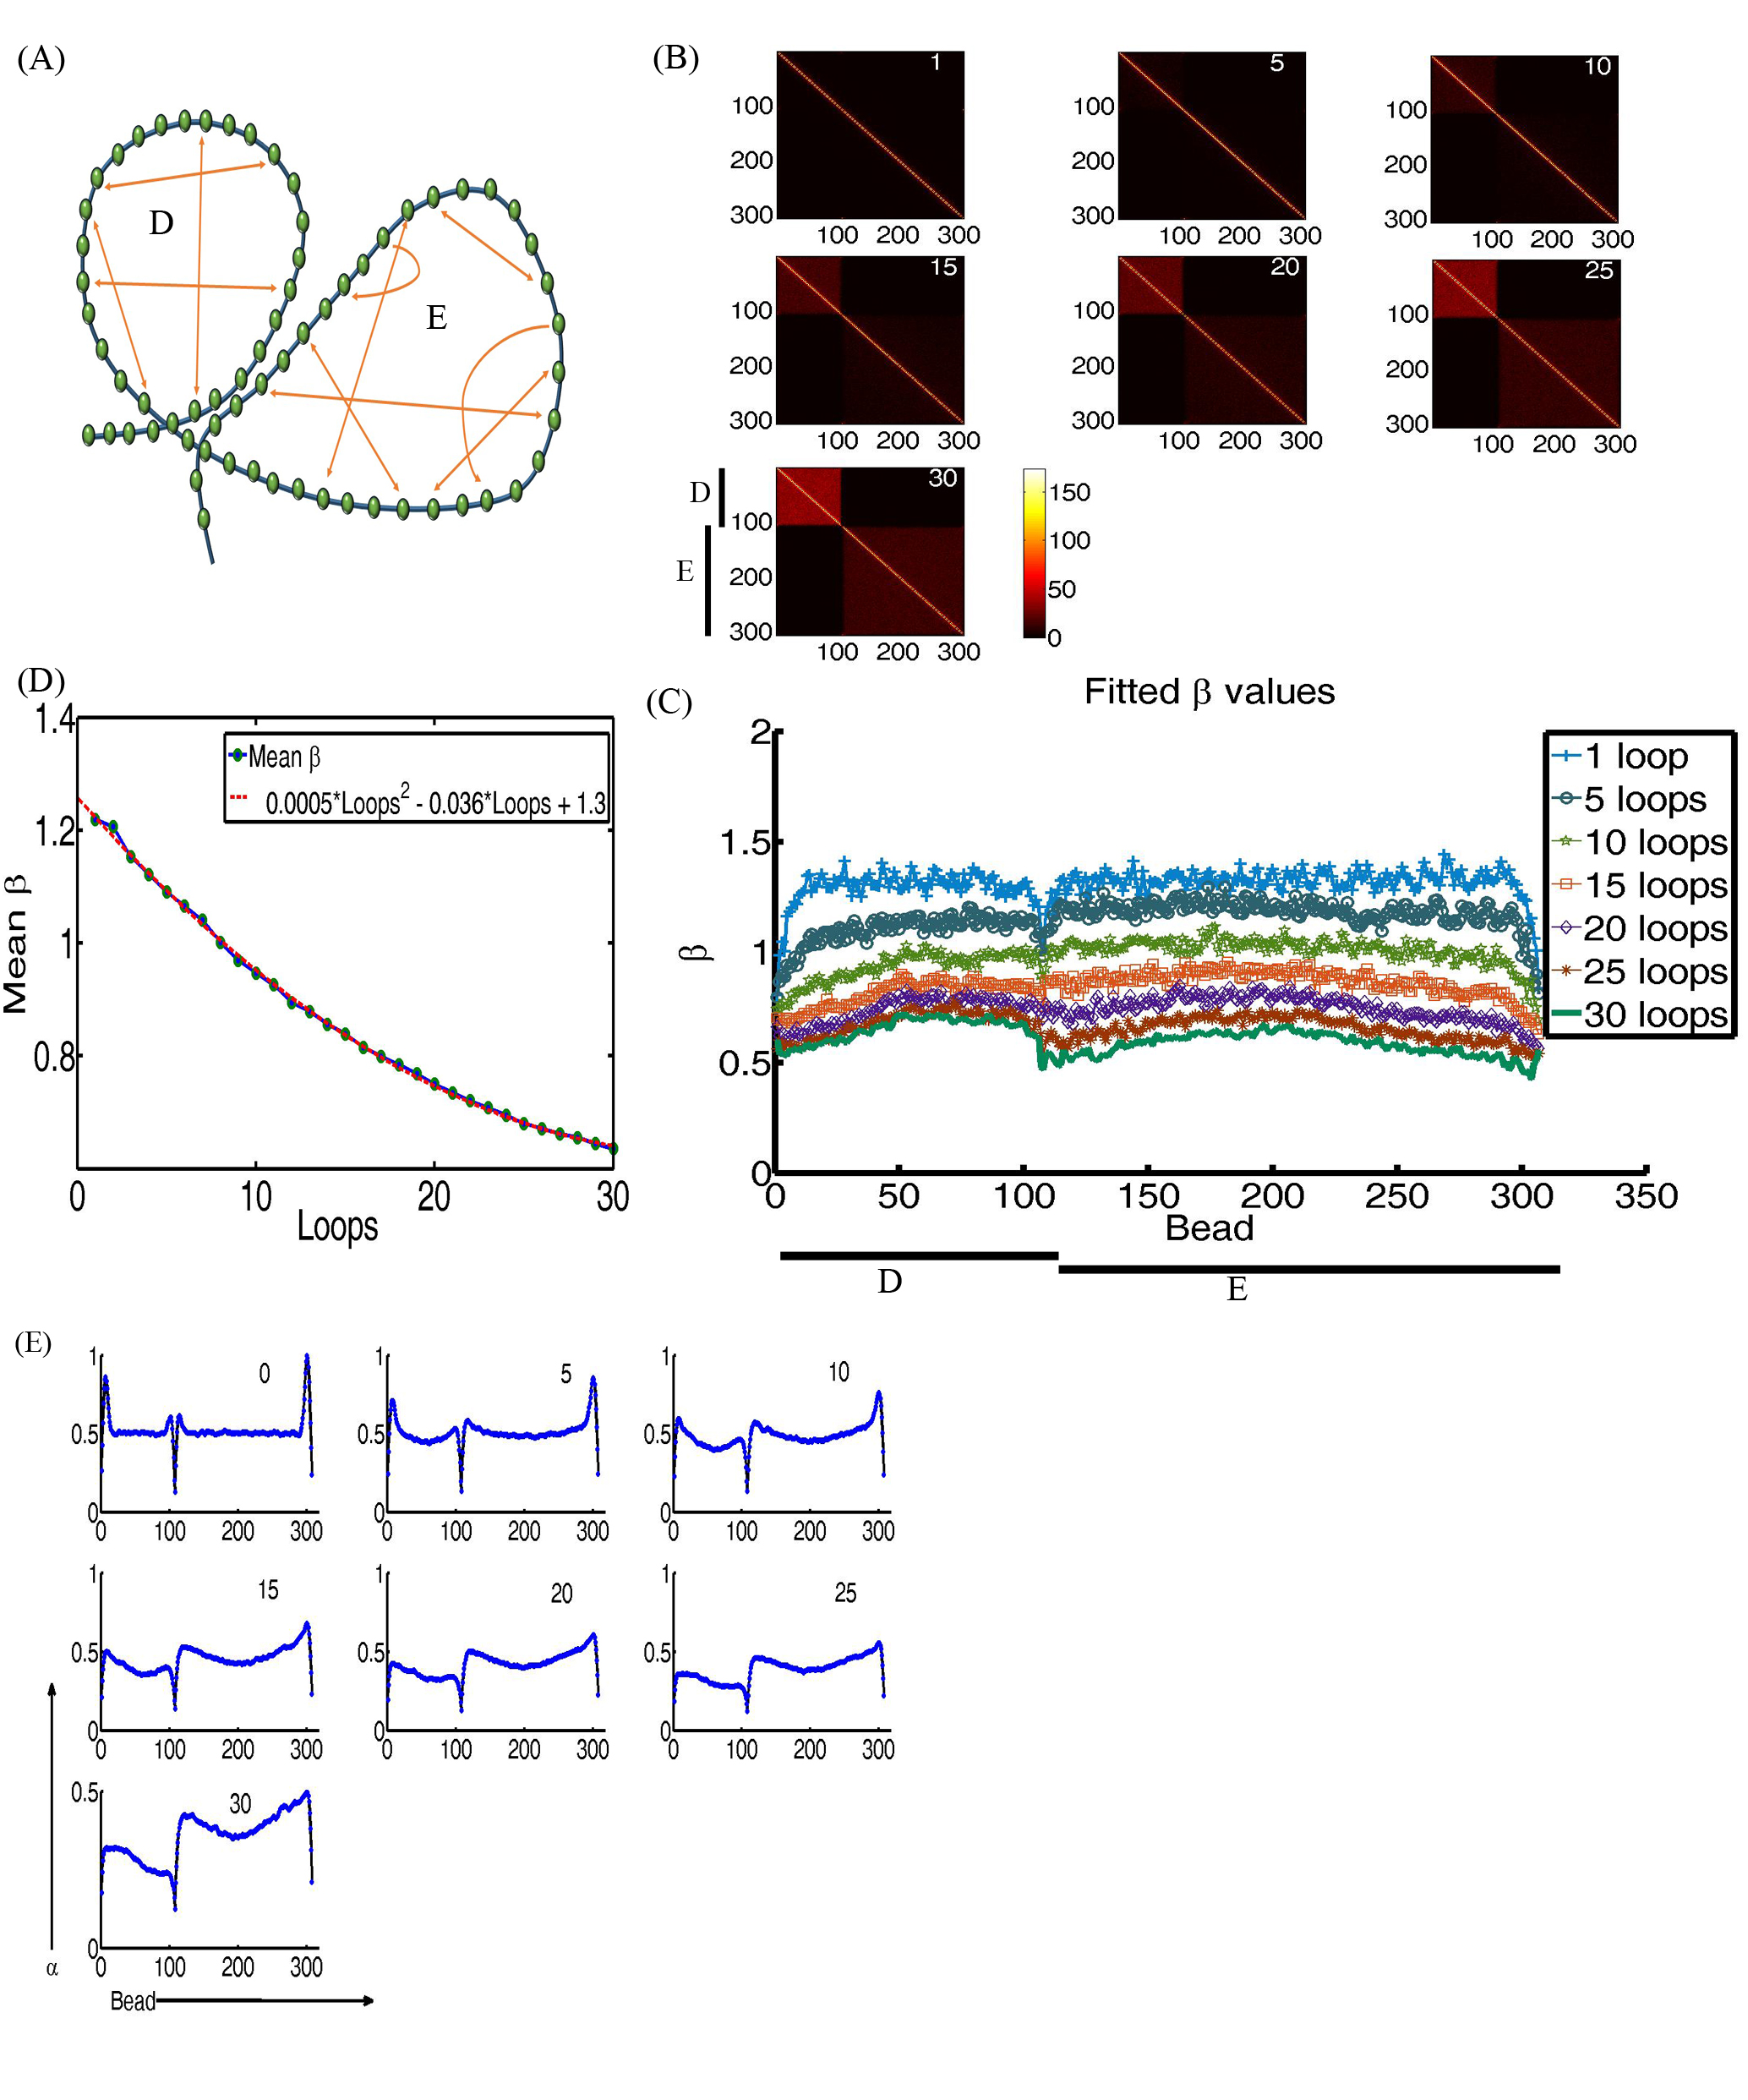
\includegraphics[scale=0.7]{Figure04_TwoTADs0To30RandomLoops307Beads}
\caption{\textbf{Encounter profile for a polymer model with two fixed loops and 1-30 random internal loops in each} (A) A sketch of the polymer model used in simulations. Beads 1, 107 and beads 108, 307 were connected to form two large loops corresponding to the positions of TAD D and E in the experimental data. One to 30 internal loops were sequentially added in each large loops. Each loop was formed by randomly picking two beads in the range 2-106 and two in the range 108-306, as in the example shown by the orange arrows (B) The encounter histograms for 7 cases of adding internal random loops in each TAD (number indicated in white in each box) resembles the TADs of the experimental data (Figure \ref{figure_TADDAndENoraEtAl2012}.(A)) as the number of random loops is increased (C) For each number of random internal loop, a model of the form $\alpha d^{-\beta}$ was fitted to the encounter probability of each bead, with $d$ the distance in bead units. Beads on the edge between the two fixed loops (e.g beads 107-8) show decrease in $\beta$ due to the high, long range encounter probability with beads participating in each fixed loop. (D) A quadratic relationship was found empirically between the number of loops and the mean $\beta$.(E) the anomalous exponen $\alpha$ extracted from the fitted mean square displacement of each bead in the case of 0 to 30 random loops in each TAD}
\label{figure_encounterProfileTwoTADs}
\end{figure}


\begin{figure}[H]
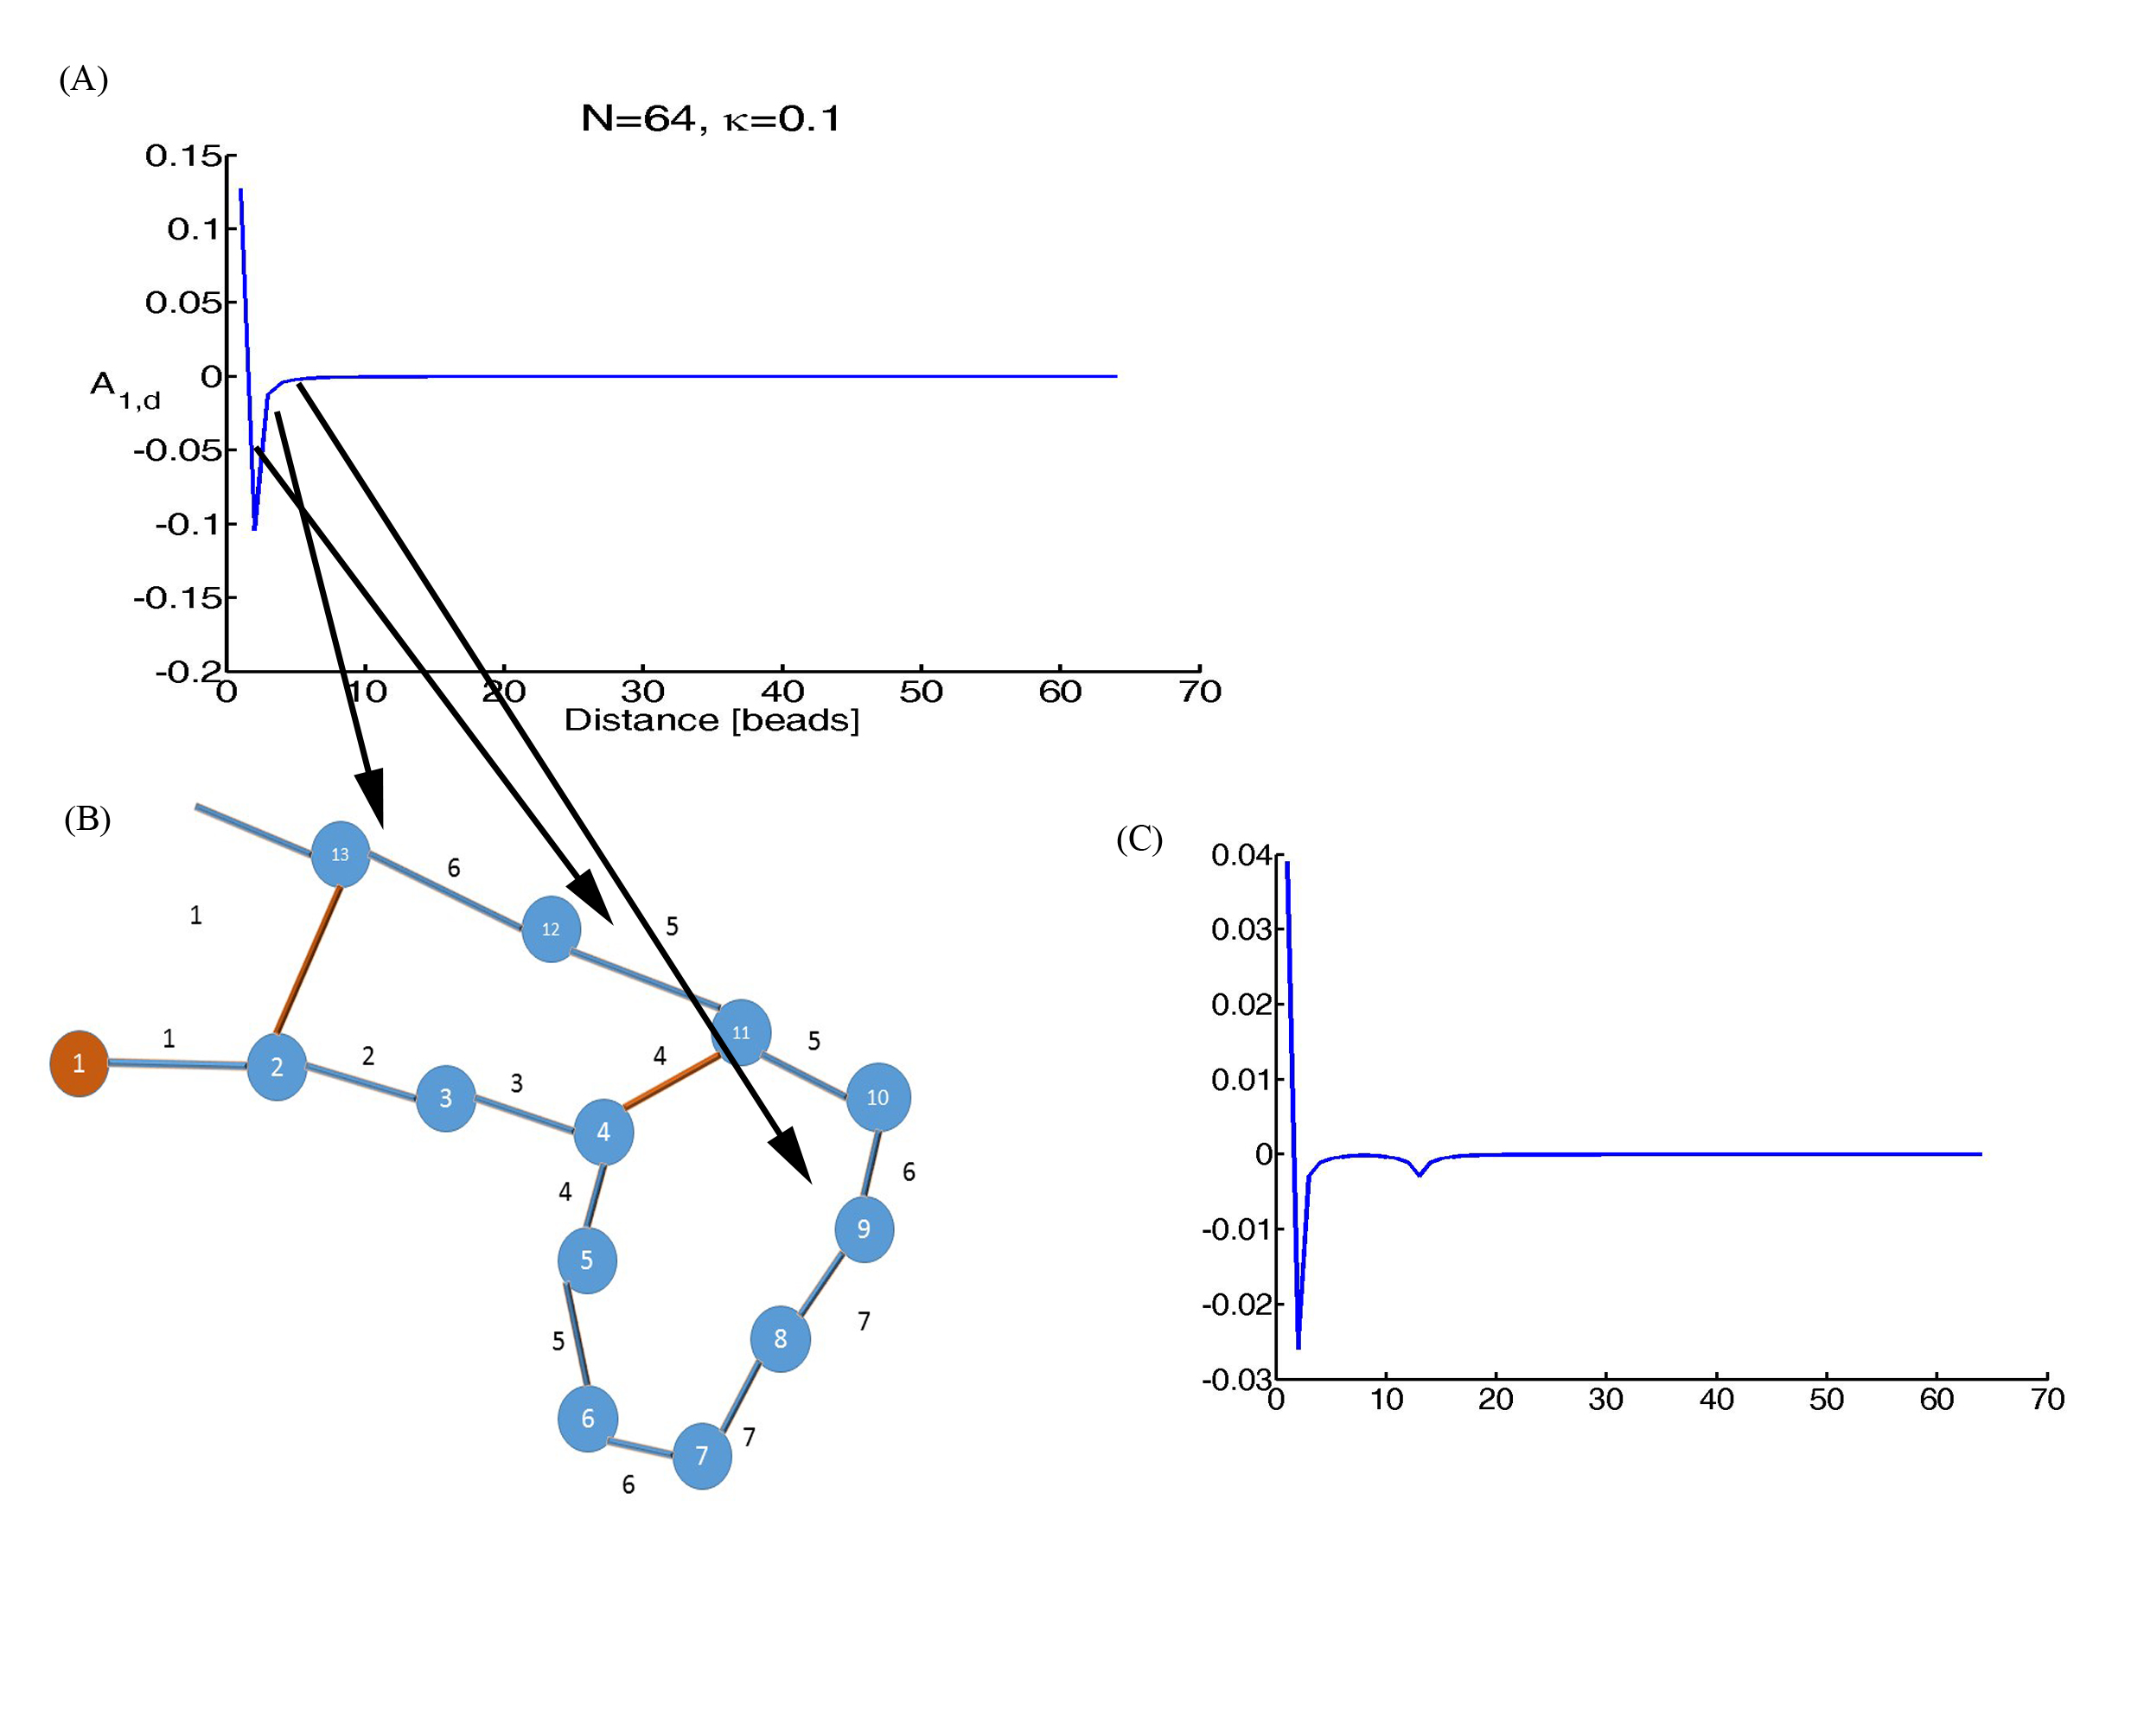
\includegraphics[scale=0.6]{Figure05_betaModelWeights}
\caption{\textbf{Setting the weights in the connectivity matrix of the $\beta$ polymer with loops}. (A) The weights in the matrix are determined by $A_{l,m}= 4\kappa \frac{2}{N}\sum_{p=1}^{N-1} sin^{\beta}(p\pi/(2N))cos((l-0.5)p\pi/N)\cos((m-0.5)p\pi/N)$, the curve is drawn for bead 1. (B) The polymer is treated as a graph with nodes representing beads (circles) and edges as springs(bars). An example of an architecture in which be beads 2 and 13 and 4 and 11 are connected (orange line). Arrows indicate that the new value for the weights for bead 1 in positions 13, 11, 9 are determined by the values of the original curve with no peaks at positions corresponding to the shortest distance between bead 1 and the rest. (C) Connecting two beads in the polymer changes the weights such that the new curve must be continuous.  New weights are assigned by the values of the $\beta$ polymer weights according to the closest distance between beads on the connected polymer graph}
\label{settingBetsModelWeights}
\end{figure}

\begin{figure}[H]
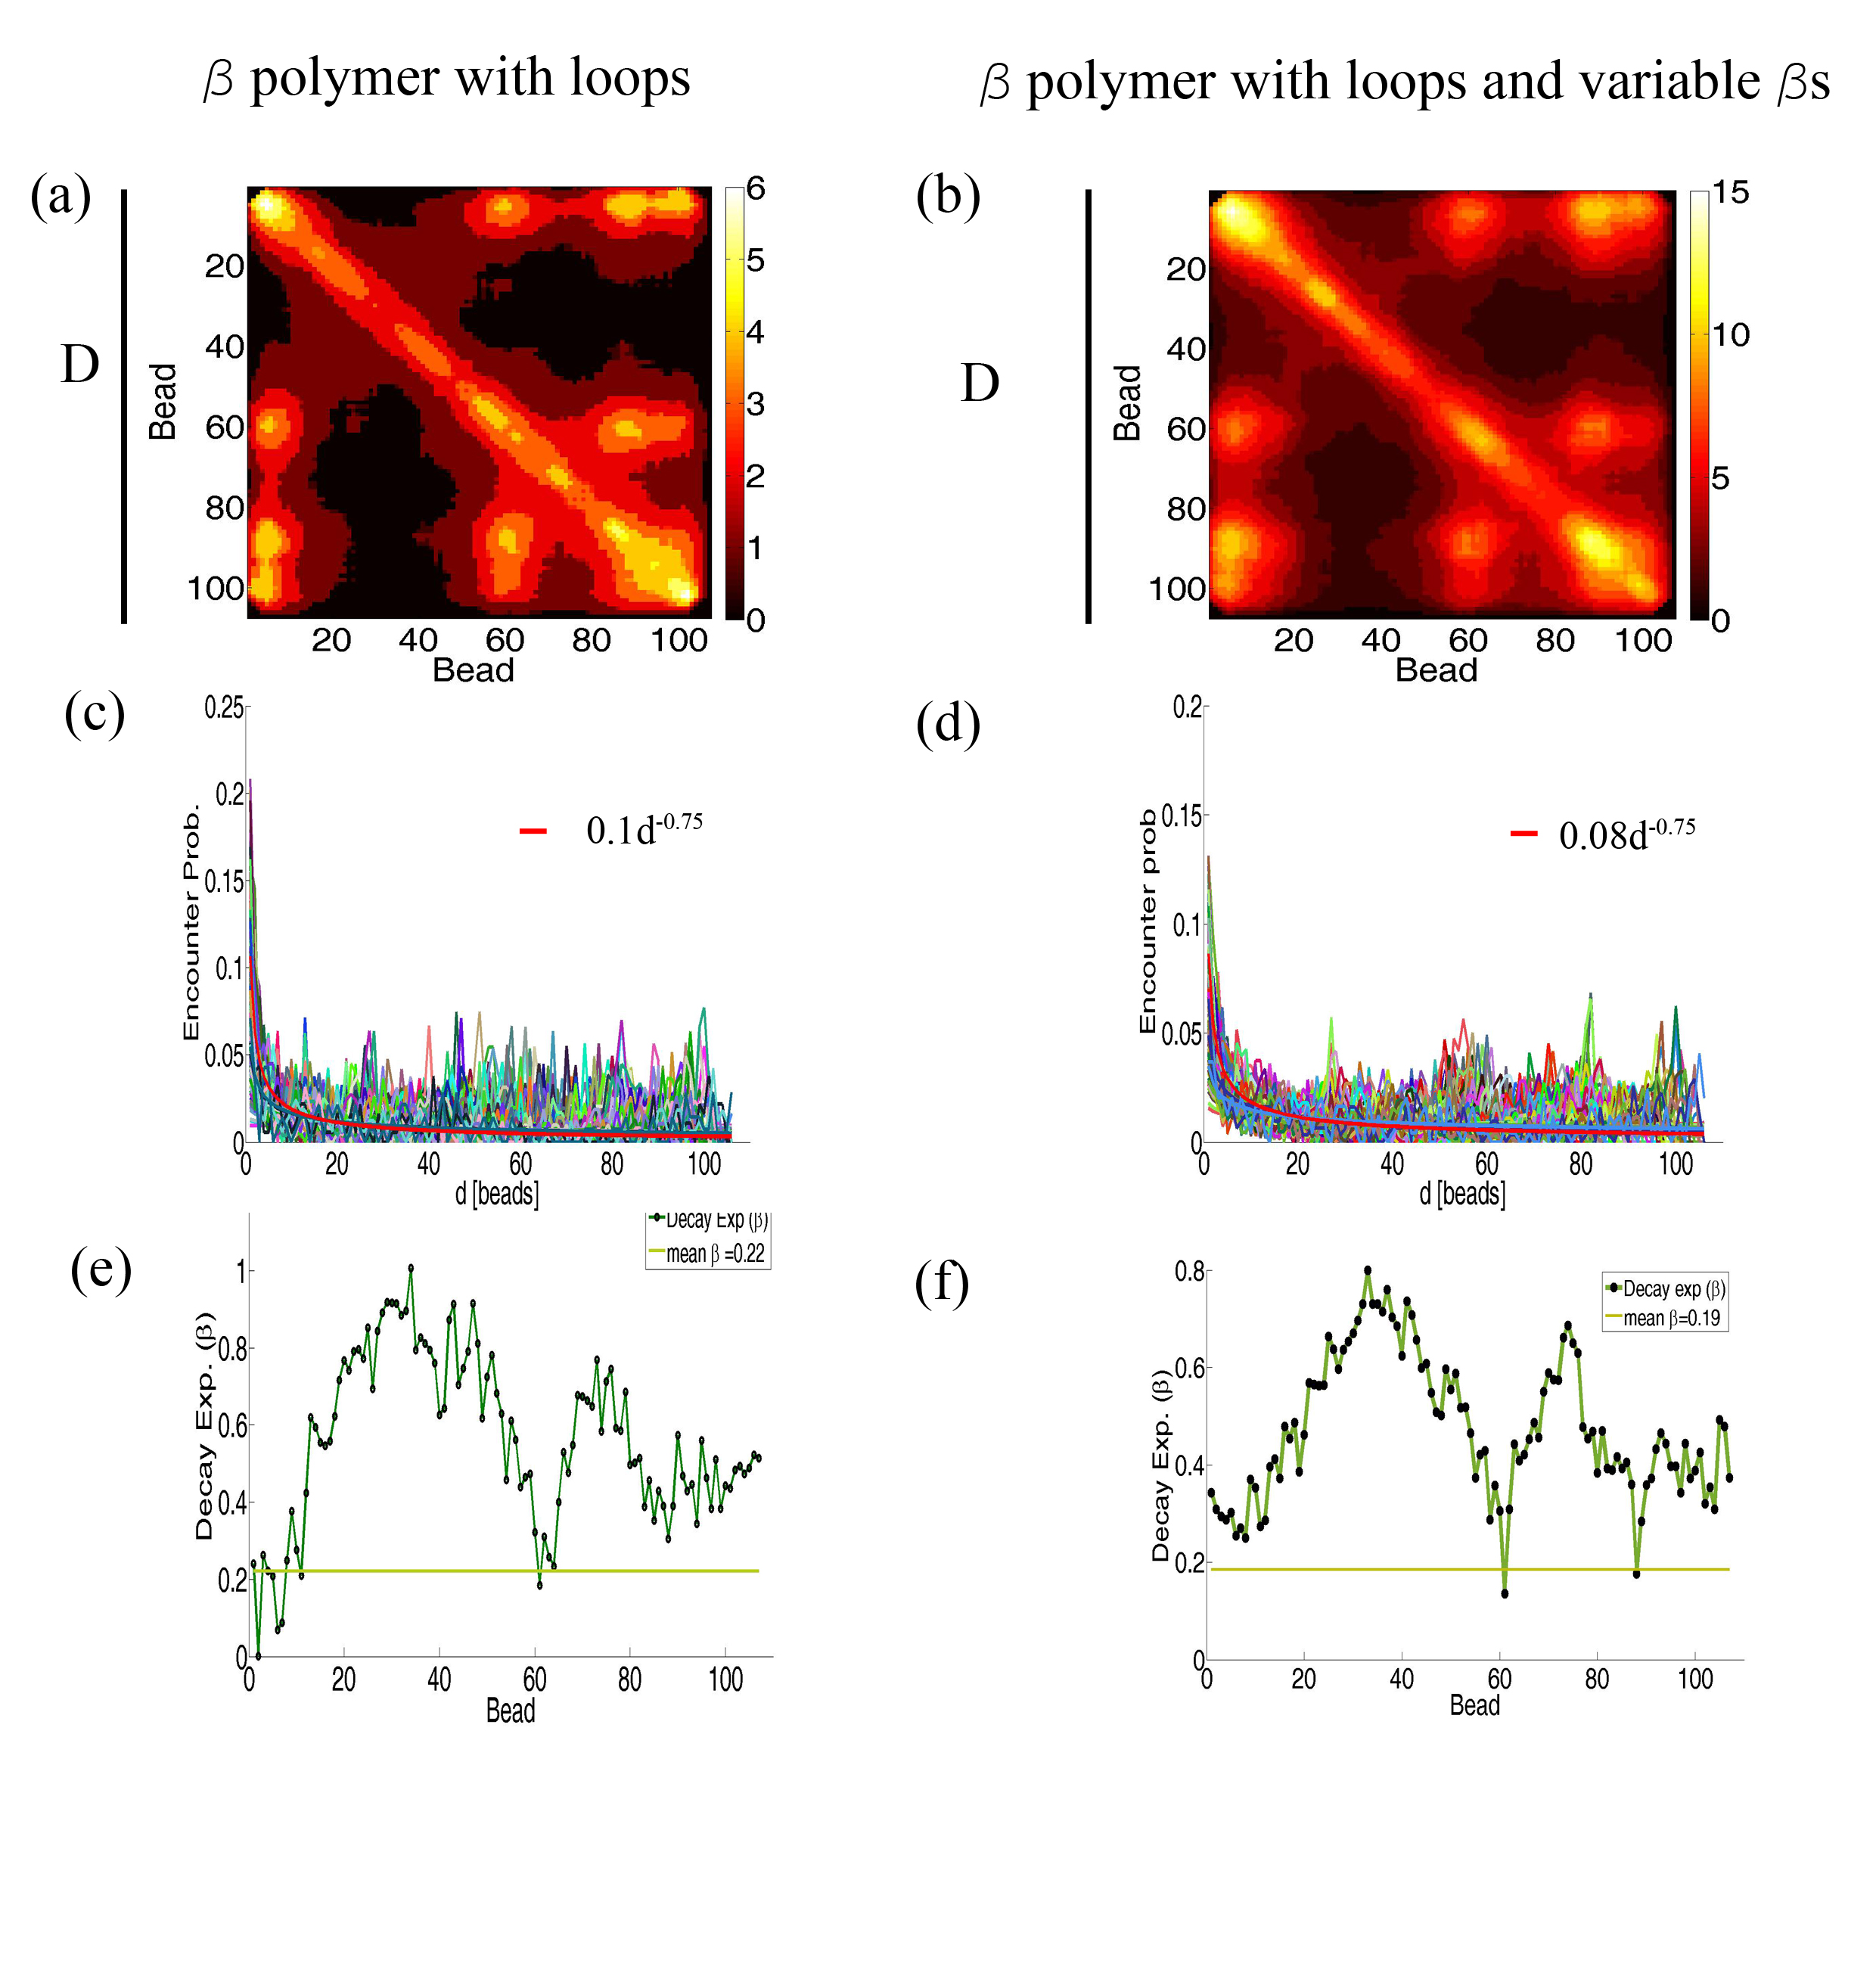
\includegraphics[scale=0.7]{Figure06_betaModelWithPeaks}
\caption{\textbf{Simulation of the $\beta$ model with loops corresponding to peaks of the encounter data}. (A) The encounter histogram of the beta model in the region of TAD D alone. The peaks were extracted using a peak calling procedures and connectors were placed between beads forming the peak of the encounter data. (B) the encounter probability of the $\beta$ model. (C) The fitted $\beta$ values of the $\beta$ model shows an unexpected behavior since in the $\beta$ model the values of the $\beta$s are constant for all beads.}
\label{simulationWithBetaPolymerWithLoops}
\end{figure}


\begin{figure}[H]
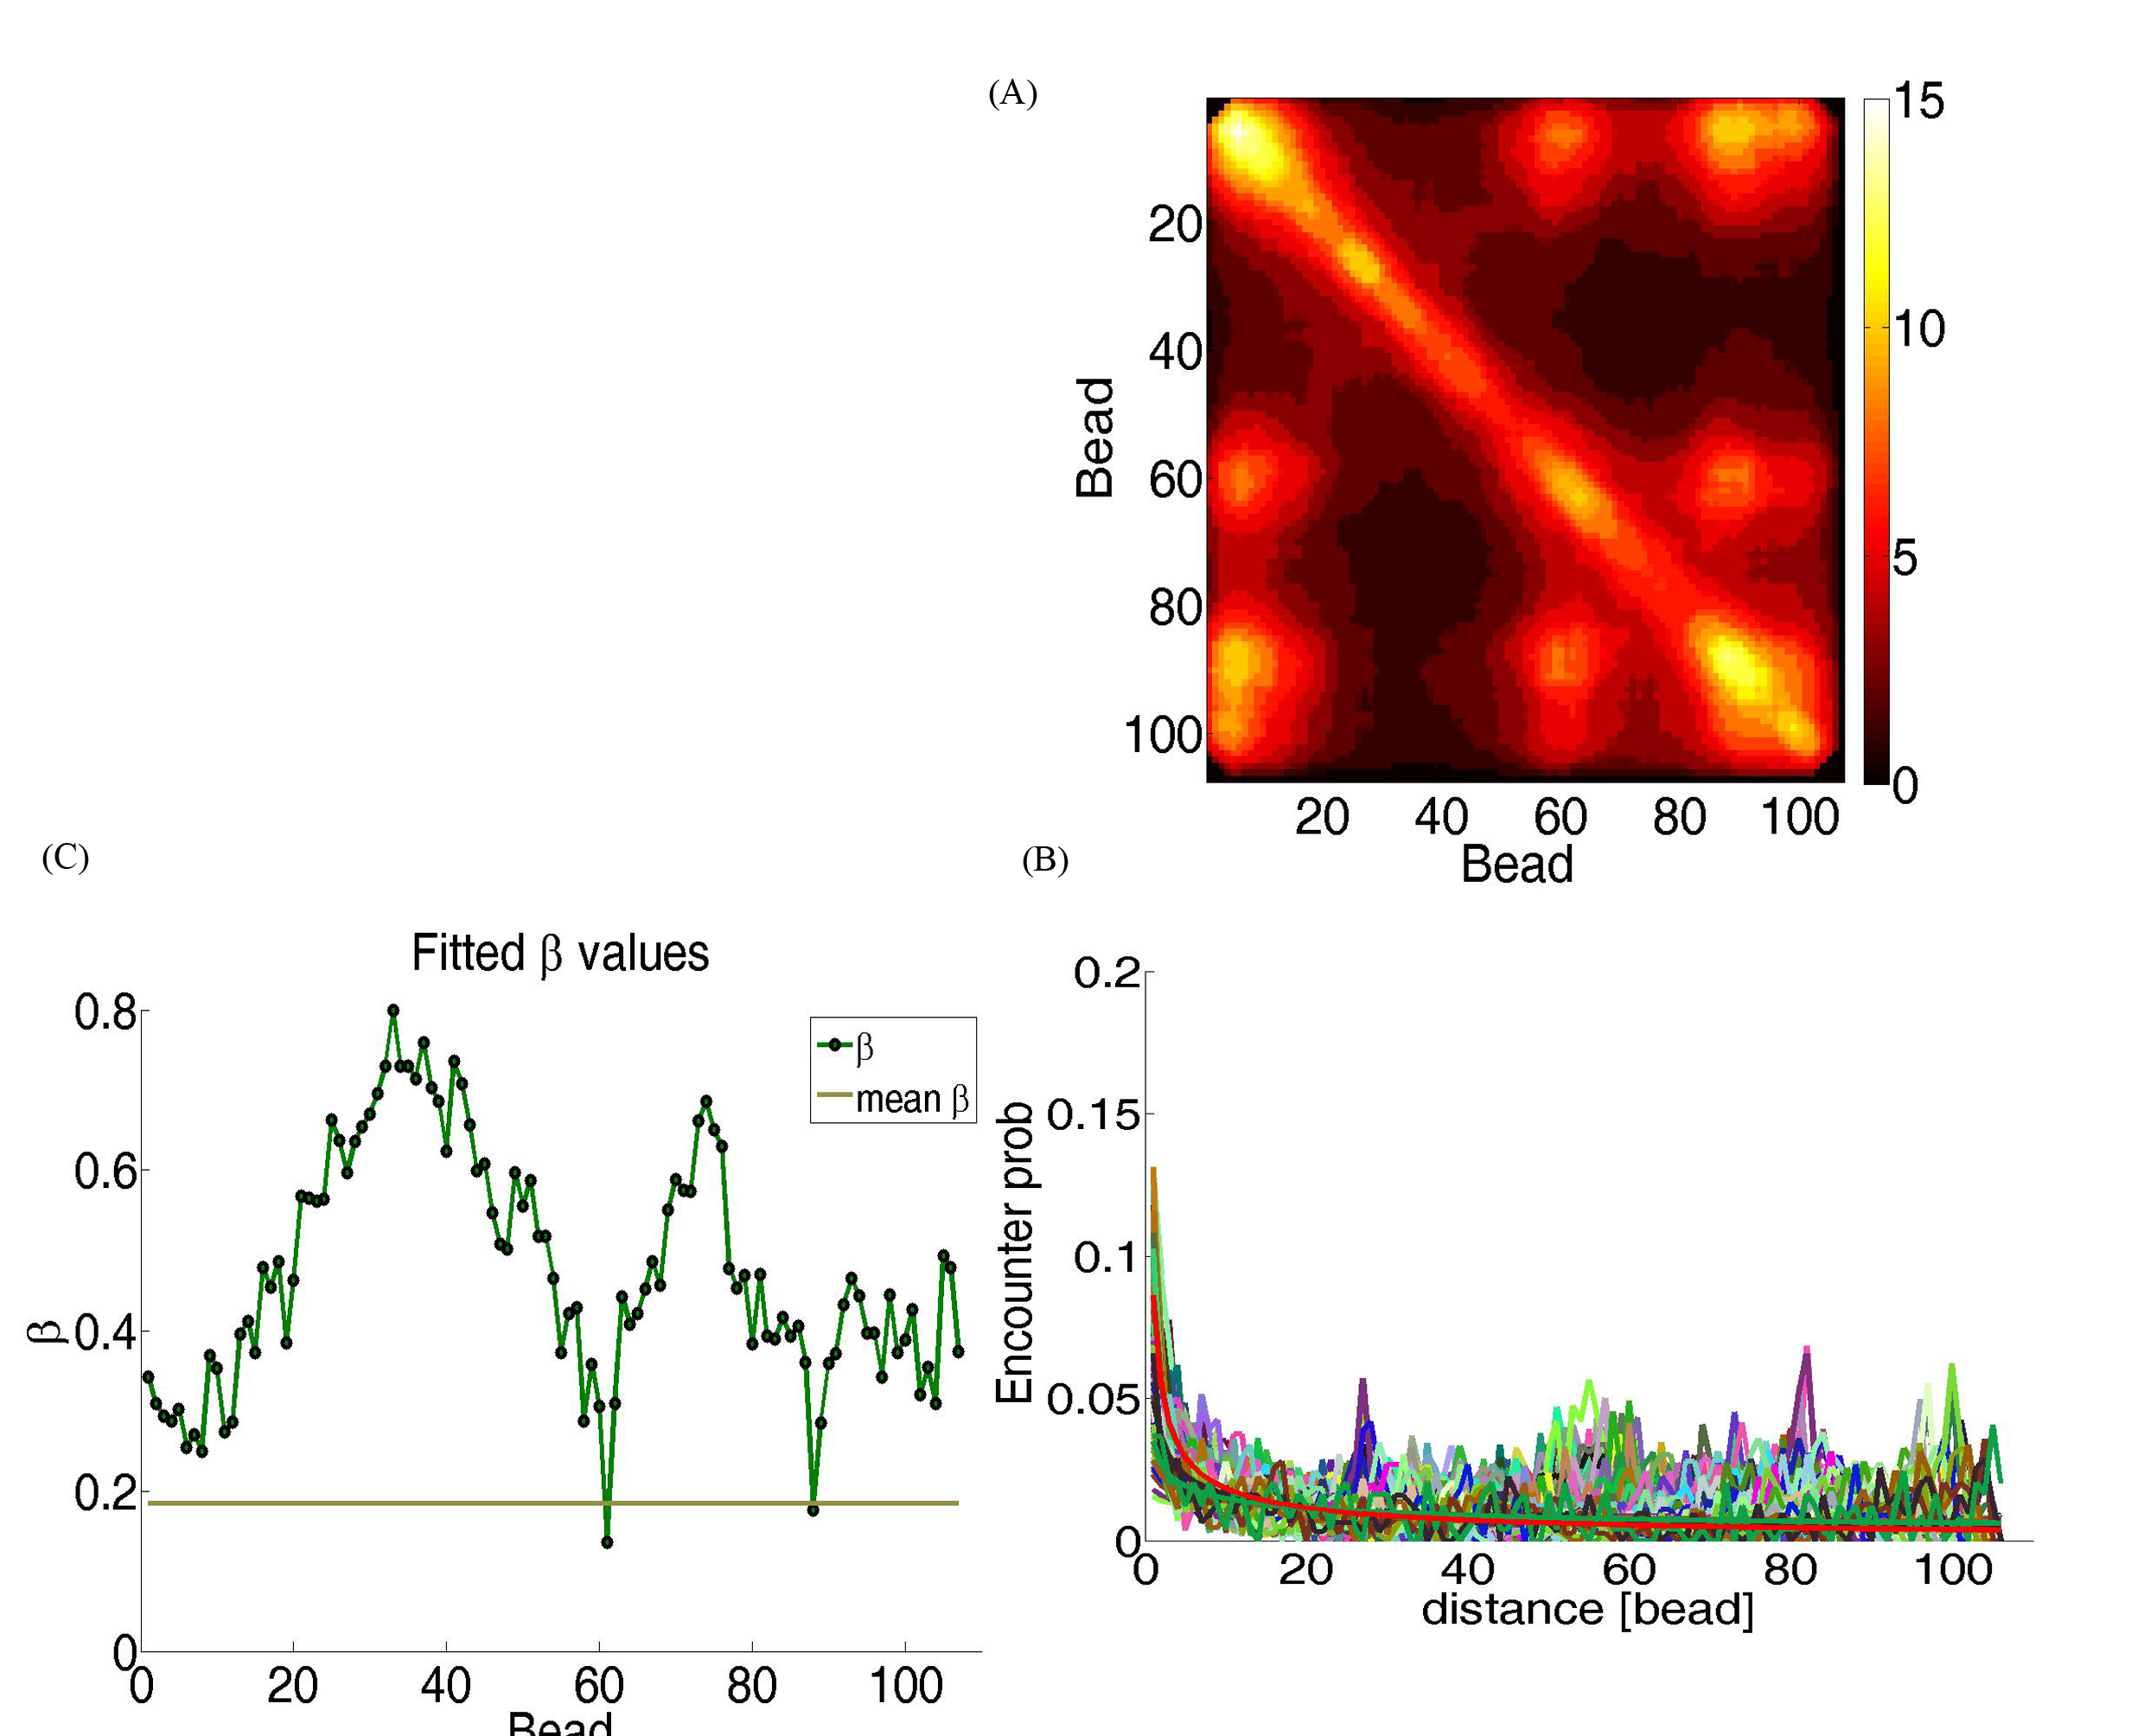
\includegraphics[scale=0.7]{Figure07_betaModelWithPeaksVariableBeta}
\caption{\textbf{Simulation of the $\beta$ model with loops corresponding to peaks of the encounter data with variable $\beta$ values}. (A) $\beta$ values for the polymer are directly determined from the encounter probability of experimental data by the model $\alpha d^{-\beta}$.}
\label{simulationWithBetaPolymerWithLoopsVariableBeta}
\end{figure}


%> the bibliography section
\bibliographystyle{plain}
\bibliography{randomLoopsBibliography} % the bibliography.bib
\end{document}

